\documentclass{beamer}

% \input{extra-tex/four-per-page.tex}

\usepackage{amssymb}
\usepackage{amsmath}
\usepackage{amsfonts}
\usepackage{listings}
\usepackage{cancel}
\usepackage{multicol}
\usepackage{multirow}

\usepackage{xcolor}
\usepackage{graphicx}
\usepackage[most]{tcolorbox}
\usepackage{textcomp} % Arrows
\usepackage{hyperref}

% Beamer stuff
\addtobeamertemplate{navigation symbols}{}{%
    \usebeamerfont{footline}%
    \usebeamercolor[fg]{footline}%
    \hspace{1em}%
    \insertframenumber/\inserttotalframenumber
}


\title{MU \LaTeX{} Workshop}
\date{2\textsuperscript{nd} May 2022}

\begin{document}
% ------------------------------------------------------------------------------ %
\begin{frame}
    \titlepage
    \center{
\includegraphics[scale=0.08]{img/MU Logo.png}}
\end{frame}
% ------------------------------------------------------------------------------ %
% ------------------------------------------------------------------------------ %

\section{Why LaTeX and what is it?}

% ------------------------------------------------------------------------------ %
\begin{frame}
    \tableofcontents
\end{frame}

\begin{frame}[fragile]{Why \LaTeX{}? Why bother with it?}
    \begin{itemize}
        \item \LaTeX{} is the gold standard for formatting maths. Many apps support LaTeX maths formatting (eg. Notion, Markdown, Discord, websites).
        \item[+] It is durable (doesn't corrupt like Word)
        \item[+] Separation of content (what you're writing) from style (how it looks)
        \begin{itemize}
            \item[+] Automatically places figures/tables, etc
            \item[+] You can swap out the styles easily
            \item[+] The styles look great by default
        \end{itemize}
        \item[+] Can easily separate out your document into manageable files (eg. for sections) 
        \item[=] Really good for academia!
        \begin{itemize} 
            \item[$\hookrightarrow{}$] 90\%+ of papers in engineering/maths/physics are written using LaTeX!
        \end{itemize} 
    
    \end{itemize}
\end{frame}

\begin{frame}[fragile]{What is \LaTeX{}?}
    \begin{itemize}
        \item \LaTeX{} vs Word
        \begin{itemize}
            \item \emph{LaTeX is a markup language} (ie. kinda like a coding language), that can be compiled to PDF by using a LaTeX engine.\\
            ``What you \textbf{mean} is what you get'' (WYMIWYG) editor
            \item \emph{Word is a visual, GUI editor.}\\
            ``What you \textbf{see} is what you get'' (WYSIWYG) editor
        \end{itemize}
        
        \item Where to write LaTeX
        \begin{itemize}
            \item Online (via. Overleaf)
            \item Locally (using MikTeX, VScode, or other)
        \end{itemize}

        \item Lay-tech?
        \begin{itemize}
            \item Valid pronunciations include `Lay-tech', `Lah-tech', or `Lay-tex'. This \href{https://tex.stackexchange.com/q/17502}{\color{blue}\underline{Stackoverflow article}} explains it
        \end{itemize}
    \end{itemize}
    
\end{frame}

\begin{frame}[fragile]{When shouldn't I use \LaTeX{}?}
    \begin{itemize}
        \item For maths working heavy documents (if you want to be time efficient)
        \begin{itemize}
            \item Maths working can take a while to set out in LaTeX, still faster to handwrite (unless you become a LaTeX god\textsuperscript{TM})
        \end{itemize}

        \item If you want absolute control over styling/positioning
        \begin{itemize}
            \item Not as much control over styling out the box. Text interface makes it difficult to see final positioning.
        \end{itemize}
    \end{itemize}
\end{frame}

\begin{frame}[fragile]{Before we start!}
    If you forget everything in this workshop, remember this!
    \begin{itemize}
        \item LaTeX Wikibook {\tiny(\url{https://en.wikibooks.org/wiki/LaTeX})}
        \begin{itemize}
            \item Amazing resource for learning LaTeX!
        \end{itemize}

        \item Detexify {\tiny(\url{https://detexify.kirelabs.org/})}
        \begin{itemize}
            \item Draw a symbol to find its LaTeX command!
        \end{itemize}
        \item Various cheat sheets online! {\tiny(\url{http://tug.ctan.org/info/undergradmath/undergradmath.pdf})}
        
    \end{itemize}
\end{frame}

% ------------------------------------------------------------------------------ %

\section{Getting started}
\begin{frame}
    \tableofcontents[currentsection]
\end{frame}
% ------------------------------------------------------------------------------ %
\begin{frame}[fragile]{\insertsection : Document Layout}
    \begin{tcblisting}{colback=red!5!white,colframe=red!75!black,listing only,left=2mm,right=2mm,title=Typical Document Set Up}
\documentclass[a4paper,14pt]{article}
% Import any packages here!    
\title{ Title }
\author{ Author }
\date{ Date }

\begin{document}

\maketitle

\section{Introduction}
Text Here!
\end{document}
    \end{tcblisting}
\end{frame}
% ------------------------------------------------------------------------------ %
\begin{frame}[fragile]{\insertsection : Reserved Characters}
    \begin{itemize}
        \item Backslash \textbackslash{} is the master key - distinguishes command from content. \textbackslash{}\textbackslash{} creates a new line.
        \item Curly brackets \{\} are used to contain and define commands
        \item Percent sign \% is used for comments
    \end{itemize}
    \begin{tabular}{r|l}
        \textbf{Special character} & \textbf{Using special character as text}\\\hline\hline
        \verb|%| & \verb|\%|\\
        \verb|$| & \verb|\$|\\
        \verb|{| or \verb|}| & \verb|\{| or \verb|\}|\\
        \verb|&| & \verb|\&|\\
        \verb|#| & \verb|\#|\\
        \verb|_| & \verb|\_|\\
        \verb|^| & \verb|\^{}|\\
        \verb|~| & \verb|\~{}|\\
    \end{tabular}
\end{frame}
% ------------------------------------------------------------------------------ %
\begin{frame}[fragile]{\insertsection : Macros and Environments}
    \begin{itemize}
        \item Commands are either macros or environments
        \item Macros
        \begin{itemize}
            \item Macros begin with \verb|\|. They may sometimes require \emph{arguments} given using curly brackets \{\} (or optional arguments in square brackets [ ])
        \end{itemize}
        \item Environments
        \begin{itemize}
            \item Surrounded by \verb|\begin{environment}|and \verb|\end{environment}|
        \end{itemize}
    \end{itemize}

    \begin{tcblisting}{colback=red!5!white,colframe=red!75!black,listing side text,left=2mm,right=2mm,title=Example 2}
\[
\left|
\begin{array}{cc}
     2-\lambda & 0\\
     4 & 3-\lambda\\
\end{array}
\right|
\]
    \end{tcblisting}
\end{frame}
% ------------------------------------------------------------------------------ %
% ------------------------------------------------------------------------------ %
\begin{frame}[fragile]{\insertsection : Packages}
    Extend base LaTeX by using packages! Adds macros and environments to your document.
    Some of the most useful to use:
    \vskip 2em
    \begin{tabular}{l|l}
        Package & Use\\
        \hline
        amsmath, amssymb, amsfonts & various maths tools \\
        geometry& to finely tune page size + margins \\
        pgfplot& to create figures and plots \\
        hyperref& to embed links \\
        graphicx& to add graphics and figures  \\
        siunitsx& for units in maths  \\
    \end{tabular}
\end{frame}
% ------------------------------------------------------------------------------ %

\section{Basic Writing}

% ------------------------------------------------------------------------------ %
\begin{frame}
    \tableofcontents[currentsection]
\end{frame}
% ------------------------------------------------------------------------------ %
\begin{frame}[fragile]{\insertsection : Text Options}
    We can change font options either using the
    \begin{enumerate}
        \item \alert{command}
        \begin{itemize}
            \item Surround small blocks of text
            \item \verb|\command{text}|
        \end{itemize}
        \item \alert{switch command}
        \begin{itemize}
            \item Convert large blocks of text
            \item Use  \verb|\switchcommand|
            \item Will keep text option unless changed or;
            \item can surround text with \verb|{\switchcommand text}|
        \end{itemize}
    \end{enumerate}
\end{frame}
% ------------------------------------------------------------------------------ %
\begin{frame}[fragile]{\insertsection : Text Options}
    Can change font size:\\
        \begin{center}
        \begin{tabular}{ll}
            \verb|\tiny|         & \tiny{Example} \\
            \verb|\scriptsize|   & \scriptsize{Example} \\
            \verb|\small|        & \small{Example} \\
            \verb|\large|        & \large{Example} \\
            \verb|\Large|        & \Large{Example} \\
            \verb|\LARGE|        & \LARGE{Example} \\
            \verb|\huge|         & \huge{Example}  \\
            \verb|\Huge|         & \Huge{Example}  \\
        \end{tabular}
        \end{center}
    Each can act as a switch command or normal command.
\end{frame}
% ------------------------------------------------------------------------------ %
\begin{frame}[fragile]{\insertsection : Text Options}
    Can change font style:\\
        \begin{center}
        \begin{tabular}{lll}
            \verb|\textbf| & \textbf{Example} & Bold\\
            \verb|\textit| & \textit{Example} & Italic\\
            \verb|\textsc| & \textsc{Example} & Small Caps\\
        \end{tabular}\\
        \end{center}
    Or font family:
        \begin{center}
        \begin{tabular}{lll}
            \verb|\textrm| & \textrm{Example} & Roman\\
            \verb|\texttt| & \texttt{Example} & Typewriter\\
            \verb|\textsf| & \textsf{Example} & Sans Serif\\
        \end{tabular}
        \end{center}
    Whose switch commands can be evoked using \verb|\rmfamily| etc.
\end{frame}
% ------------------------------------------------------------------------------ %
\begin{frame}[fragile]{\insertsection : Text Options}
    Can change font colour:
    \begin{tcblisting}{colback=red!5!white,colframe=red!75!black,left=2mm,right=2mm,title=Changing Text Colour}
Here is how you can change the colour of single \textcolor{red}{words} using the command, or changing { \color{red} blocks of texts by surrounding it in curly brackets } using the switch command.
    \end{tcblisting}
The package xcolor is particularly useful for getting very specific colours.
\end{frame}
% ------------------------------------------------------------------------------ %
\begin{frame}[fragile]{\insertsection : Lists}
    \begin{itemize}
        \item We can make ordered and unorded lists using the following environments:
            \begin{enumerate}
                \item \verb|\begin{enumerate}| for unordered lists
                \item \verb|\begin{itemize}| for ordered lists
                \item \verb|\begin{description}| for long paragraphs
            \end{enumerate}
        \item Each point is denoted using the \verb|\item| command
        \item You can nest up to four lists
        \item[:)] You can change the bullet by specifying it as an argument in \verb|\item[new bullet]|
    \end{itemize}
\end{frame}
% ------------------------------------------------------------------------------ %
\begin{frame}[fragile]{\insertsection : Lists}
    \begin{tcblisting}{colback=red!5!white,colframe=red!75!black,left=2mm,listing only,right=2mm,title=Example List}
\begin{itemize}
    \item Heres an example of a list!
        \begin{enumerate}
            \item And how you can nest lists!
            \item Of any kind!
        \end{enumerate}
    \item[!] And how you can change bullet points
    \end{itemize}
    \end{tcblisting}
\end{frame}
% ------------------------------------------------------------------------------ %

\section{Formatting Documents}

% ------------------------------------------------------------------------------ %
\begin{frame}
    \tableofcontents[currentsection]
\end{frame}
% ------------------------------------------------------------------------------ %
\begin{frame}[fragile]{\insertsection : Title Pages}
    \begin{itemize}
        \item We can make a title with \verb|\maketitle| with the various options we give it
            \begin{itemize}
                \item \verb|\title{}|
                \item \verb|\author{}|
                \item \verb|\date{}|
            \end{itemize}
        \item A page of contents with \verb|\tableofcontents|
        \item An abstract using \verb|\begin{abstract}| environment
        \item Further customisation using \verb|\begin{titlepage}| environment
    \end{itemize}
\end{frame}
% ------------------------------------------------------------------------------ %
\begin{frame}[fragile]{\insertsection : Sections}
    Heirarchy of \LaTeX{} is always important
    \begin{enumerate}
        \item \verb|\section{}|
        \item \verb|\subsection{}|
        \item \verb|\subsubsection{}|
    \end{enumerate}
    We can suppress numbering putting an asterix after the command, such as \verb|\section*{}|
\end{frame}
% ------------------------------------------------------------------------------ %
\begin{frame}[fragile]{\insertsection : Spacing}
    \begin{itemize}
        \item Kerning exists
        \item \verb|\,|, \verb|\:|, \verb|\;|, \verb|\!| and \verb|\ | (with a space) give increasing spaces between words
        \item \verb|\quad| gives space equal to current font size (from the quadrat!)
        \item \verb|\vspace{<length>}| and \verb|hspace{<length>}|
        \item \verb|\\| ends the line and starts another
        \item \verb|\newline| will insert a new line altogether
        \item \verb|\newpage|
    \end{itemize}
\end{frame}
% ------------------------------------------------------------------------------ %

\section{Mathematics}

% ------------------------------------------------------------------------------ %
\begin{frame}
    \tableofcontents[currentsection]
\end{frame}
% ------------------------------------------------------------------------------ %
\begin{frame}[fragile]{\insertsection : Environments}
    \begin{itemize}
        \item Instead of writing in \emph{text} mode, we write in \emph{math} mode
    \end{itemize}
    \begin{table}[]
        \centering
        \begin{tabular}{c||c|c|c}
            & Inline & Block equation \\
            \hline
            TeX (outdated) & \$ \$ & \$\$ \$\$ \\
            LaTeX & \verb|\( \)| & \verb|\[ \]| & \\
            Environment & \verb|\begin{math}| & \verb|\begin{displaymath}|\\
        \end{tabular}
    \end{table}
    \vskip 2ex
    \begin{itemize}
        \item We can do multi-line equations using the \verb|align| environment.
        \item \verb|\[ \]| will not number equations, \verb|\begin{equation}| will (we can suppress numbering using \verb|\begin{equation*}|, but might as well use \verb|displaymath| at that point)
    \end{itemize}
\end{frame}
% ------------------------------------------------------------------------------ %
\begin{frame}[fragile]{\insertsection : Environments}
    \begin{tcblisting}{colback=red!5!white,colframe=red!75!black,left=2mm,right=2mm,title=Inline and Oneline}
An example of inline math to write
\(\phi=2\sin(\theta)\). Or an equation like:
\[ x=\frac{-b \pm \sqrt{ b^2-4ac }}{2a}\]
    \end{tcblisting}
\end{frame}
% ------------------------------------------------------------------------------ %
\begin{frame}[fragile]{\insertsection : Environments}
    \begin{tcblisting}{colback=red!5!white,colframe=red!75!black,left=2mm,right=2mm,title=Multiline}
And a multi-line math environment such as
\begin{align*}
    0 &= x^2 - 1\\
    0 &= (x-1)(x+1)
\end{align*}
    \end{tcblisting}
\end{frame}
% ------------------------------------------------------------------------------ %
\begin{frame}[fragile]{\insertsection : Symbols}
    \begin{itemize}
        \item Symbols are accessed via macros
        \item Greek symbols:
        \begin{itemize}
            \item \verb|\Omega| for uppercase $\Omega$
            \item \verb|\omega| for lowercase $\omega$
        \end{itemize}
        \item \href{http://tug.ctan.org/info/undergradmath/undergradmath.pdf}{\color{blue}\underline{Cheat sheet!}} You'll learn them eventually
        \item Some of my most common
    \end{itemize}
    \begin{center}
        \begin{tabular}{cl|cl}
            $\int_{-1}^{1}$ &  \verb|\int_{-1}^{1}| & $\sum_{n=1}^\infty$ & \verb|\sum_{n=1}^\infty|\\
            $\frac{a}{b}$ &  \verb|\frac{a}{b}| & $\times$ & \verb|\times|\\
            $\partial$ & \verb|\partial| & $\cdots$ & \verb|\cdots|\\
            $\pm$ & \verb|\pm| & $\leq$ & \verb|\leq|\\
        \end{tabular}
    \end{center}
\end{frame}
% ------------------------------------------------------------------------------ %
\begin{frame}[fragile]{\insertsection : Superscripts and Subscripts}
    \begin{itemize}
        \item we use $\_$ and $\wedge$
        \item delimit its use with curly brackets \{ \} if more than one character is used
        \begin{tcblisting}{colback=red!5!white,colframe=red!75!black,left=2mm,right=2mm,title=Multiline}
We can add subscripts like $x_i$ or $x_{i+1}$ \\
Or superscripts like $a^2$ and $a^{n+1}$ \\
Both can be used in conjunction like $a_n^i$ \\
But this can be improved using curly brackets as 
well; ${a_n}^i$
    \end{tcblisting}
    \end{itemize}
\end{frame}
% ------------------------------------------------------------------------------ %
\begin{frame}[fragile]{\insertsection : Operators}
    \begin{itemize}
        \item $\sin, \cos, \tan$ use \verb|\sin, \cos, \tan| in math mode
        \item \verb|\frac{}{}| creates a fraction
        \item \verb|\dfrac{}{}| will force a \emph{display style} fraction
        \item \verb|\sqrt[]{}| will create a square root by default, or $nth$ root if specified in [ ]
        \item \verb|\mathop{dx}| $\mathop{dx}$ for upright differential operators if you care
        \item \verb|\text{}| to write text in math mode
    \end{itemize}
    \vskip 2ex
    \begin{tcblisting}{colback=red!5!white,colframe=red!75!black,left=2mm,right=2mm,title=Various Operators}
$ \hat{a},  \dot{a},  \ddot{a},  \bar{a} $
    \end{tcblisting}
\end{frame}
% ------------------------------------------------------------------------------ %
\begin{frame}[fragile]{\insertsection : Delimiters}
    Along with the standard delimiters found on the keyboard,
    \vskip 2ex
    \begin{center}
    \begin{tabular}{c|l}
        $\langle$ & \verb|\langle|\\
        $\rangle$ & \verb|\rangle|\\
        $\{$      & \verb|\{|\\
        $\}$      & \verb|\}|\\
        $\|$      & \verb|\mid|\\
    \end{tabular}
    \end{center}
\end{frame}
% ------------------------------------------------------------------------------ %
\begin{frame}[fragile]{\insertsection : Delimiters}
    \begin{itemize}
        \item We can use \emph{delimiters} to surround various expressions
        \item \verb|\left<delimiter>| and \verb|\right<delimiter>| to wrap using a delimiter
        \item Must have both commands to wrap
        \item use \verb|\left.| if you do not want a left delimiter (or vice versa)
    \begin{tcblisting}{colback=red!5!white,colframe=red!75!black,left=2mm,right=2mm,title=Delimiters}
\[   f(x,y)=\left\|  \frac{x+y}{2}  \right\|   \]
    \end{tcblisting}
    \end{itemize}
\end{frame}
% ------------------------------------------------------------------------------ %
\begin{frame}[fragile]{\insertsection : Delimiters}
    \begin{itemize}
        \item You can manually set the size of delimiters to distinguish nested equations
    \end{itemize}
    \begin{tcblisting}{colback=red!5!white,colframe=red!75!black,left=2mm,right=2mm,title=Delimiter Size}
\[ \big( \Big( \bigg( \Bigg(  \]
    \end{tcblisting}
\end{frame}
% ------------------------------------------------------------------------------ %
\begin{frame}[fragile]{\insertsection : Delimiters}
    \begin{tcblisting}{colback=red!5!white,colframe=red!75!black,left=2mm,right=2mm,title=Delimiter Size Example}
\[ \Big( 2\times \big( f(x,y)+g(x,y) \big) \Big)^2 \]
    \end{tcblisting}
\end{frame}
% ------------------------------------------------------------------------------ %

\section{Alignment and Arrays}

% ------------------------------------------------------------------------------ %
\begin{frame}
    \tableofcontents[currentsection]
\end{frame}
% ------------------------------------------------------------------------------ %
\begin{frame}[fragile]{\insertsection : Align}
\begin{itemize}
    \item The master key for alignment is the \&
    \item In the \verb|\begin{align}| environment, we can use it to align equations
    \item We separate lines using the \verb|\\| macro
\end{itemize}
    \begin{tcblisting}{colback=red!5!white,colframe=red!75!black,left=2mm,right=2mm,title=Alignment}
                \begin{align*}
                    0 &= x^2+x\\
                    0 &= x(x+1)\\
                    \implies x &= 0, x=-1
                \end{align*}
    \end{tcblisting}
\end{frame}
% ------------------------------------------------------------------------------ %
\begin{frame}[fragile]{\insertsection : Arrays}
\begin{itemize}
    \item \verb|\begin{array}{}| command
    \item takes alignment argument (c,l,r)
    \item each cell is separated by the \&
    \item each line is separated by the \verb|\\|
    \item we can use delimiters to form varying matrices!
    \item Array writes in math mode
\end{itemize}
\end{frame}
% ------------------------------------------------------------------------------ %
\begin{frame}[fragile]{\insertsection : Arrays}
    \begin{tcblisting}{colback=red!5!white,colframe=red!75!black,listing side text,left=2mm,right=2mm,title=Example 2}
\[
\left(
\begin{array}{cc}
     2-\lambda & 0\\
     4 & 3-\lambda\\
\end{array}
\right)
\]
    \end{tcblisting}
\end{frame}
% ------------------------------------------------------------------------------ %
\begin{frame}[fragile]{\insertsection : Matrix environments}
    We can also use \verb|pmatrix| and \verb|bmatrix| environments:
    \begin{tcblisting}{colback=red!5!white,colframe=red!75!black,listing side text,left=2mm,right=2mm,title=Example 2}
\[
\begin{pmatrix}
     2-\lambda & 0\\
     4 & 3-\lambda\\
\end{pmatrix}
\]
\[
\begin{bmatrix}
     2-\lambda & 0\\
     4 & 3-\lambda\\
\end{bmatrix}
\]
    \end{tcblisting}
\end{frame}
% ------------------------------------------------------------------------------ %
\begin{frame}[fragile]{\insertsection : Tables}
    \begin{itemize}
        \item the text mode version is \verb|\begin{tabular}{}|
        \item also takes an alignment argument
        \begin{itemize}
            \item \verb|l| \textrightarrow{} Left align
            \item \verb|c| \textrightarrow{} Centre align
            \item \verb|r| \textrightarrow{} Right align
        \end{itemize}
        \item \verb|\hline| to make horizontal breaks
        \item Extended table use
        \begin{itemize}
            \item \verb|\usepackage{booktabs}| \textrightarrow{} fancy rulings
            \item \verb|\usepackage{multicol}| and \verb|\usepackage{multirow}| \textrightarrow{} Merged cells
        \end{itemize}
        
    \end{itemize}
    \end{frame}
    % ------------------------------------------------------------------------------ %
    \begin{frame}[fragile]{\insertsection : Tables}
        \begin{tcblisting}{colback=red!5!white,colframe=red!75!black,left=2mm,right=2mm,title=Table example}
    \begin{tabular}{l|c|r} % |'s -> vertical lines
        \textbf{l align column} & \textbf{c align column} & \textbf{r align column}\\
        \hline\hline
        1 & 2 & 3\\
        4 & 5 & 6\\
        \hline
    \end{tabular}
        \end{tcblisting}
    \end{frame}
% ------------------------------------------------------------------------------ %

\section{Figures}

% ------------------------------------------------------------------------------ %
\begin{frame}
    \tableofcontents[currentsection]
\end{frame}
% ------------------------------------------------------------------------------ %
\begin{frame}[fragile]{\insertsection : Floats}
\begin{itemize}
    \item Floats cannot be broken across pages
    \item \LaTeX{} will place floats \emph{for} you where it makes sense
    \item Do not try to move floats to exactly where you want them - \LaTeX{} knows best!
    \item \verb|\begin{tabular}| environments can be put into a \verb|\begin{table}| to float
\end{itemize}
\end{frame}
% ------------------------------------------------------------------------------ %
\begin{frame}[fragile]{\insertsection : Graphics}
\begin{itemize}
    \item we use \verb|\usepackage{graphicx}| to import PNG,JPEG and PDFs
    \item \verb|\includegraphics[parameters]{file path}|
    \begin{itemize}
        \item \verb|scale=|
        \item \verb|width=|
        \item \verb|height=|
        \item \verb|angle=|
    \end{itemize}
    \item \verb|\paperwidth|, \verb|\textwidth|, \verb|cm| and \verb|in| are super useful
    \begin{itemize}
        \item \verb|width=0.8\textwidth|
        \item \verb|width=0.5\paperwidth|
        \item \verb|width=5cm|
    \end{itemize}
    \item I would recommend putting your graphics into folders
\end{itemize}
\end{frame}
% ------------------------------------------------------------------------------ %
\begin{frame}[fragile]{\insertsection}
\begin{itemize}
    \item We can specify figures using the \verb|\begin{figure}[]| environment
    \item Everything inside our environment will be floated
    \item Figures can take placement parameters
    \begin{itemize}
        \item[h] Try to place exactly here
        \item[t] Try to place on top of page
        \item[b] Try to place at bottom of page
        \item[p] Place on separate page only for floats
    \end{itemize}
    \item You can put as many as you want, and \LaTeX{} will go through them one by one
\end{itemize}
\end{frame}
% ------------------------------------------------------------------------------ %
\begin{frame}[fragile]{\insertsection}
\begin{itemize}
    \item Commonly used with \verb|\centering|
    \item \verb|\caption{}|
    \item \verb|\label{}| can be used to reference your figure
\end{itemize}
    \vskip 2ex
    \begin{tcblisting}{colback=red!5!white,colframe=red!75!black,listing only,left=2mm,right=2mm,title=Default Figure}
\begin{figure}
    \centering
    \includegraphics{}
    \caption{Caption}
    \label{fig:my_label}
\end{figure}
    \end{tcblisting}
\end{frame}
% ------------------------------------------------------------------------------ %
\begin{frame}[fragile]{\insertsection : Referencing Figures}
\begin{itemize}
    \item We can use \verb|\ref{label}| to call any figure or table
    \item \LaTeX will count figures and tables separately
    \item The same can be done with equations if you label them (they will also be counted separately)
\end{itemize}
\end{frame}
% ------------------------------------------------------------------------------ %
\begin{frame}[fragile]{\insertsection : Arranging Figures}
\begin{itemize}
    \item If you'd like to arrange figures in a specific way, you can use \verb|\begin{minipage}{width}|
    \item \verb|minipages| will align themselves next to each other if there is no whitespace
    \item perfect solution for arrays of figures
\end{itemize}
\begin{figure}[h]
    \begin{minipage}{4cm}
        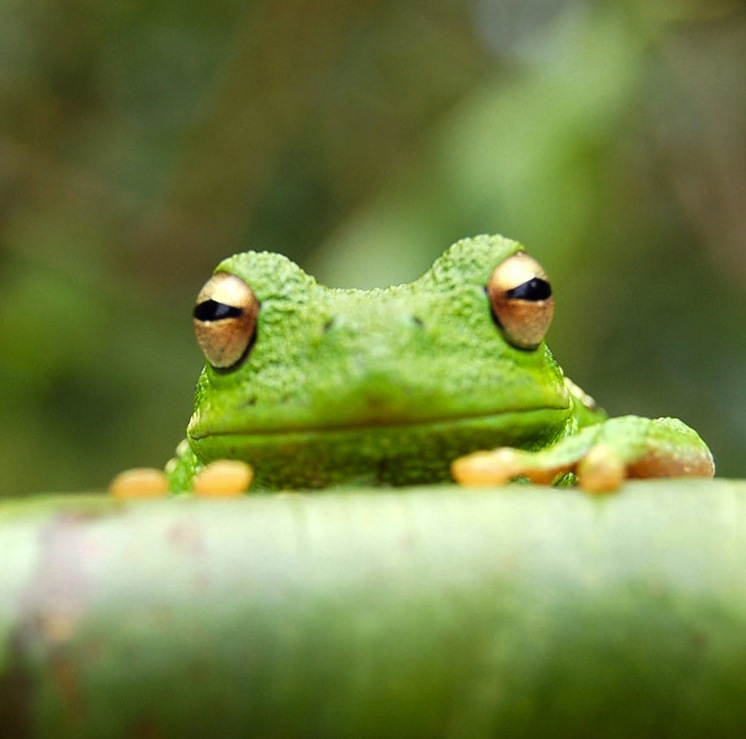
\includegraphics[width=4cm]{img/frog.jpg}
    \end{minipage}
    \begin{minipage}{4cm}
        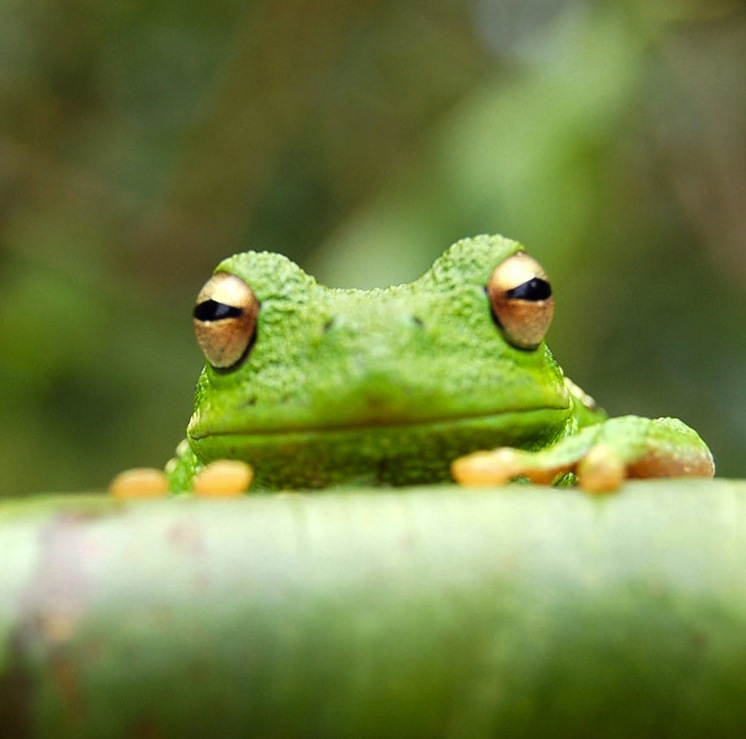
\includegraphics[width=4cm]{img/frog.jpg}
    \end{minipage}
    \caption{Frogs (2).}
\end{figure}
\end{frame}
% ------------------------------------------------------------------------------ %
\begin{frame}[fragile]{\insertsection : Arranging Figures}
The source code for the previous figure:
    \begin{tcblisting}{colback=red!5!white,colframe=red!75!black,listing only,left=2mm,right=2mm,title=Frogs Figure}
\begin{figure}[h]
    \begin{minipage}{4cm}
        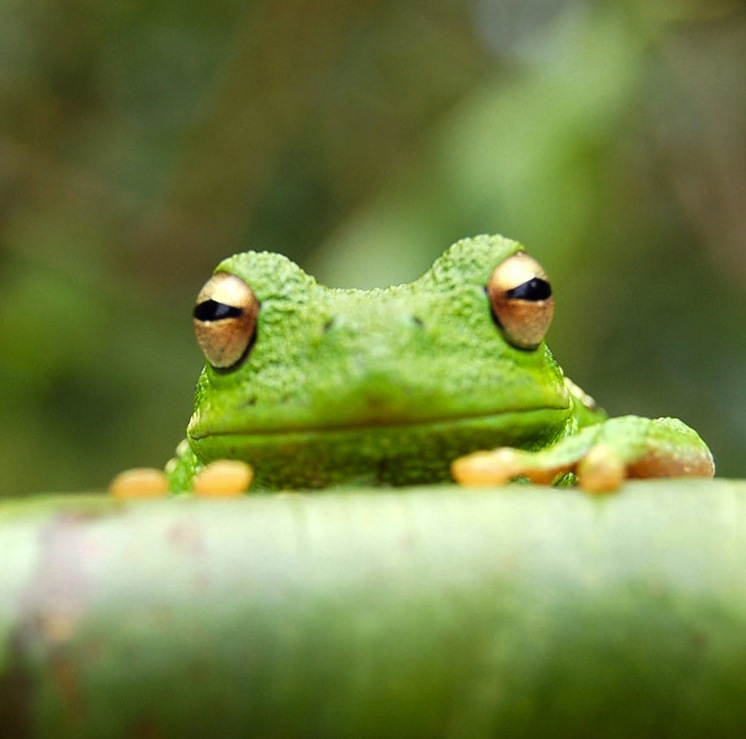
\includegraphics[width=4cm]{img/frog.jpg}
    \end{minipage}
    \begin{minipage}{4cm}
        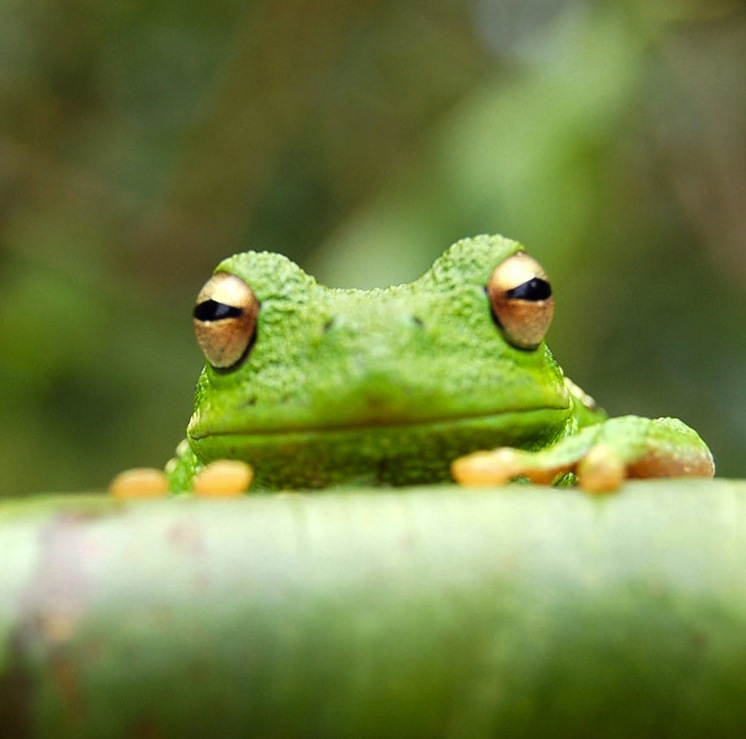
\includegraphics[width=4cm]{img/frog.jpg}
    \end{minipage}
    \caption{Frogs (2).}
\end{figure}
    \end{tcblisting}
\end{frame}
% ------------------------------------------------------------------------------ %

\section{Concluding Remarks}

% ------------------------------------------------------------------------------ %
\begin{frame}
    \tableofcontents[currentsection]
\end{frame}
% ------------------------------------------------------------------------------ %
\begin{frame}[fragile]{\insertsection : What Now?}
\begin{itemize}
    \item Practice!
    \item Explore new packages that may be of use to you
    \begin{itemize}
        \item pgfplots
        \item tikz
        \item booktabs - lots more
        \item mhchem - for chemical equations'
        \item biblatex - referencing
    \end{itemize}
    \item \url{https://tex.stackexchange.com/}
\end{itemize}
\end{frame}
% ------------------------------------------------------------------------------ %
\begin{frame}[fragile]{\insertsection : What Now?}
\begin{itemize}
    \item Tinker with other built in commands and formatting tools
    \item Make your own commands and macros
    \begin{itemize}
        \item \verb|\newcommand{}[]{}|
        \item \verb|\newcommand{\R}{\mathbb{R}}|
        \item \verb|\newcommand{\deriv}[1]{\frac{d}{d#1}}|
    \end{itemize}
\end{itemize}
\end{frame}
% ------------------------------------------------------------------------------ %
% \begin{frame}[fragile]{\insertsection : Feedback}
% If you could scan the QR code below to give feedback, that would be great.
% \end{frame}
% ------------------------------------------------------------------------------ %
\begin{frame}[fragile]{}
\center{Thank You!}
\end{frame}


\end{document}